\section{Icecube Basics}

\tdplotsetmaincoords{60}{110}
%
\pgfmathsetmacro{\rvec}{3}
\pgfmathsetmacro{\thetavec}{40}
\pgfmathsetmacro{\phivec}{60}

\begin{frame}{Neutrinos}
    \begin{columns}
        \begin{column}{0.4\textwidth}
            \begin{itemize}
                \item They come in three flavors: $\nu_{\mathbb{e}}, \nu_{\mathbb{\mu}}, \nu_{\mathbb{\tau}}$
                \item They are uncharged
                \item They only via the weak force
                \item \emph{Very light}: $m_{\nu} < \SI{0.8}{\electronvolt}$\footnotemark[1]
                \item \emph{Very hard} to observe
                \item[$\Rightarrow$] There is still a lot to learn about and from neutrinos!
            \end{itemize}
        \end{column}
        \begin{column}{0.6\textwidth}
            \begin{figure}
                \centering
                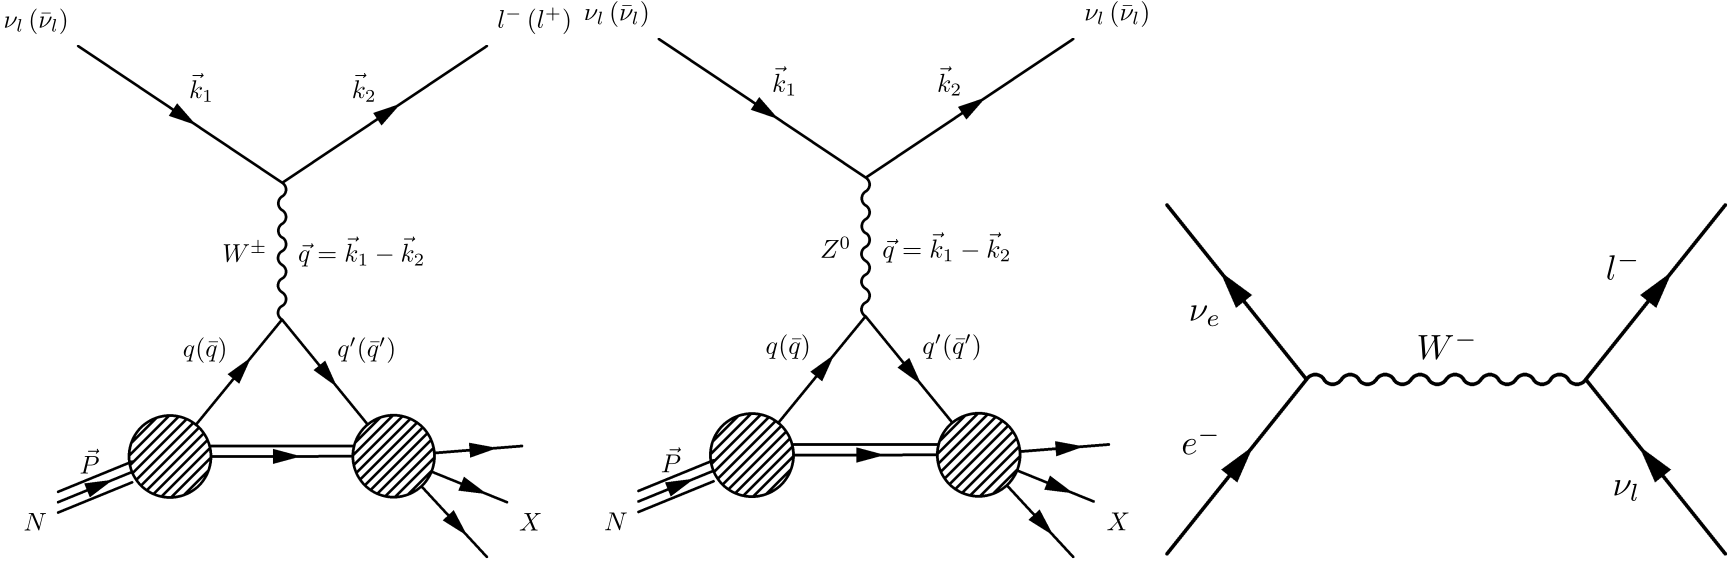
\includegraphics[width=\textwidth]{media/feynman_diagrams.png}

                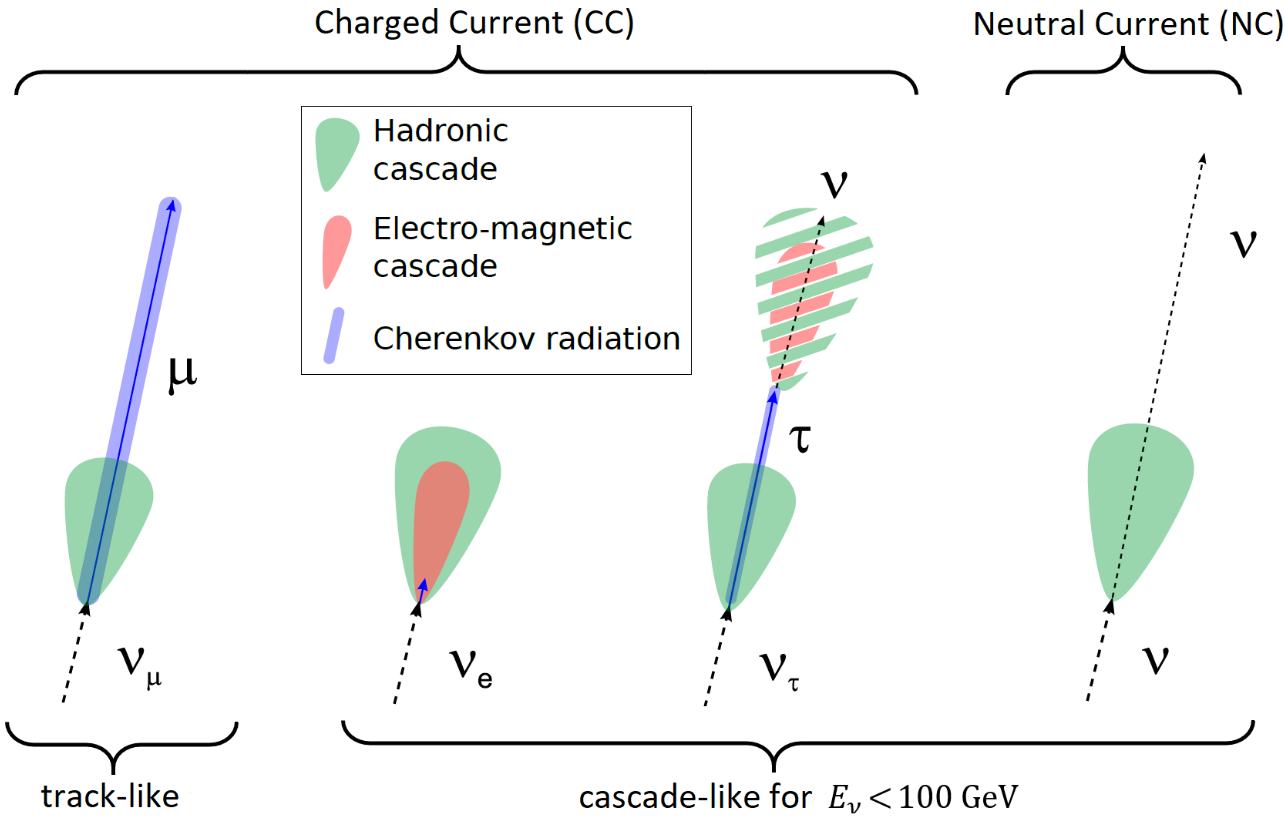
\includegraphics[width=.6\textwidth]{media/neutrino_interaction.png}
                \caption*{Feynman Diagrams and interaction signatures at Icecube \footnotemark[2]}
            \end{figure}
        \end{column}
    \end{columns}
    \footnotetext[1]{{\fullcite{aker2022direct}}}
    \footnotetext[2]{{\fullcite{reimann2020search}}}
\end{frame}
\begin{frame}{The Icecube Observatory\dots}
    \begin{columns}
        \hspace{-3em}
        \begin{column}{.6\textwidth}
            \vspace{-2em}
            \begin{figure}
                \centering
                \begin{tikzpicture}[tdplot_main_coords]
                    \node at (0, 0){
                        \def\svgwidth{1\textwidth}
                        \graphicspath{{media/}}
                        \fontsize{6}{4}\selectfont
                        \input{media/icecube_opt.pdf_tex}
                    };
                \end{tikzpicture}
                \vspace{-2em}
                \caption*{\small Modified from \fullcite{reimann2020search} }
            \end{figure}
        \end{column}
        \hspace{-2em}
        \begin{column}{.4\textwidth}
            \begin{itemize}
                \item[\textbf{\dots}] is located at the South-Pole.
                \item[\textbf{\dots}] finished construction in 2010.
                \item[\textbf{\dots}] has \SI{1}{\kilo\meter\tothe{3}} total volume.
                \item[\textbf{\dots}] can detect (InIce): $E_{\nu} = \mathcal{O}\l(\unit{\tera\electronvolt}\r)-\mathcal{O}\l(\unit{\peta\electronvolt}\r)$.
                \item[\textbf{\dots}] can detect (DeepCore): $E_{\nu} > \SI{10}{\giga\electronvolt}$.
            \end{itemize}
        \end{column}
        \hspace{2em}
    \end{columns}
\end{frame}

\begin{frame}{The Icecube Observatory Vocabulary}
    \begin{columns}
        \hspace{-3em}
        \begin{column}{.6\textwidth}
            \vspace{-2em}
            \begin{figure}
                \centering
                \begin{tikzpicture}[tdplot_main_coords]
                    \node at (0, 0){
                        \def\svgwidth{1\textwidth}
                        \graphicspath{{media/}}
                        \fontsize{6}{4}\selectfont
                        \input{media/icecube_opt.pdf_tex}
                    };
                    \coordinate (O) at (2,2.5,3.5);
                    \draw[thick,->] (O) -- +(2,0,0) node[anchor=north east, shift={(-.2,.1)}]{\small$x$};
                    \draw[thick,->] (O) -- +(0,2,0) node[anchor=west]{\small$y$};
                    \draw[thick,->] (O) -- +(0,0,2) node[anchor=east]{\small$z$};
                    \tdplotsetcoord{P}{\rvec}{\thetavec}{\phivec}
                    \draw[stealth-,color=mLightBrown] (O) -- +(P) node[above right] {$\nu$};
                    \draw[dashed, color=mLightBrown] (O) -- +(Pxy);
                    \draw[dashed, color=mLightBrown] (O)+(P) -- +(Pxy);
                    \tdplotdrawarc{(O)}{1}{0}{\phivec}{anchor=south, shift={(.2,-.1)}}{\small$\phi$}
                    \tdplotsetthetaplanecoords{\phivec}
                    \tdplotdrawarc[tdplot_rotated_coords]{(O)}{1}{0}%
                    {\thetavec}{anchor=north,shift={(0,-.1)}}{\small$\theta$}
                \end{tikzpicture}
                \vspace{-2em}
                \caption*{\small Modified from \fullcite{reimann2020search} }
            \end{figure}
        \end{column}
        \hspace{2em}
        \begin{column}{.4\textwidth}
            \begin{itemize}
                \item [\textbf{Zenith}] $\theta$
                \item [\textbf{Azimuth}] $\phi$
                      \pause
                \item [\textbf{DOM}] Digital-Optical-Module (PMT)
                \item [\textbf{InIce}] 78 strings\\ each 60 DOMs\\ DOM-to-DOM: \SI{17}{\meter}
                      string-to-string: \SI{125}{\meter}
                \item [\textbf{Deep Core}] 8 high efficiency strings
                      string-to-string: \SI{75}{\meter}
                      \pause
                \item [\textbf{$\hookrightarrow$Upper}]  10 DOMS, DOM-to-DOM: \SI{10}{\meter}
                \item [\textbf{$\hookrightarrow$Lower}]  50 DOMS, DOM-to-DOM: \SI{7}{\meter}
            \end{itemize}
        \end{column}
        \hspace{-2em}
    \end{columns}
\end{frame}
\begin{frame}{Methods of Reconstruction}
    \centering
    \begin{columns}[T]
        \begin{column}{.25\textwidth}
            LineFit\\
            \begin{equation*}
                \min_{\vec{x}_0, \vec v} \sum_{i=1}^{N}\abs{\vec x_i - \l(\vec{x}_{0}+\vec v t_i\r)}^2
            \end{equation*}
            \begin{itemize}
                \item Minimize square error
                \item Simple first guess
                \item Not much physics \enquote{input}
            \end{itemize}
        \end{column}
        \pause
        \begin{column}{.35\textwidth}
            MPEFit\\
            \begin{equation*}
                \max_{\vec{r}_0, t_0, \phi, \theta} \prod_{i=1}^{N} p\l(t_{i,\mathrm{res}}\middle|\vec{r}_0, t_0, \vec d(\phi, \theta)\r)
            \end{equation*}
            \begin{itemize}
                \item Maximize Likelihood $\mathcal L$
                \item Complex
                \item A lot of physics input
                \item Uncertainty by varying $\mathcal L$(Paraboloid)
            \end{itemize}
        \end{column}
        \pause
        \begin{column}{.4\textwidth}
            Machine Learning \\
            \begin{equation*}
                \min_{\vec p} \frac{1}{N}\sum_{i=1}^{N} L(y_{\mathrm{pred}}=\hat{f}\l(\mathbf{X_i} \middle | \vec p\r), y_{i,\mathrm{true}})
            \end{equation*}

            \begin{itemize}
                \item Minimize empirical loss-function $\mathbf L$
                \item Training the $\vec p$ is complex, but applying is simple
                \item No physics input, except true label $y_{i,\mathrm{true}}$
                \item Uncertainty from estimator $\hat f$
            \end{itemize}
        \end{column}
    \end{columns}
\end{frame}
\begin{frame}{Monte Carlo Simulation}
    From where do we get the true labels, e.g $E, \theta$ or $\phi$?
    $\rightarrow$ \textbf{Monte Carlo Simulation} \\
    \vspace{1em}
    \begin{center}
        Generate Primary Particle ($E_\nu, \theta, \phi$)\\
        $\downarrow$\\
        Propagation/Interaction/Decay
        \\$\downarrow$\\
            Detector interaction and response (DOM pulses)
            \\$\downarrow$\\
        Machine Learning input (e.g. $n$ features per DOM)
    \end{center}
    \pause
    \textbf{Do we trust our simulation data?}
\end{frame}